\documentclass[12pt, a4paper]{article}

\usepackage[utf8]{inputenc}

% Limit the page margin to only 1 inch.
\usepackage[margin=1in]{geometry}

%Imports biblatex package
\usepackage[
backend=biber,
style=alphabetic
]{biblatex}
\addbibresource{../math-342w.bib}

% Enables the `align' environment.
\usepackage{amsmath}
\allowdisplaybreaks
\usepackage{bm}
\usepackage{array}
\usepackage{rotating}
\usepackage{multirow}

% Provides useful environments, such as:
% - \begin{proof} ...\end{proof}
\usepackage{amsthm}
\newtheorem{proposition}{Proposition}
\theoremstyle{definition}
\newtheorem*{definition}{Definition}
\newtheorem{theorem}{Theorem}
\newtheorem{corollary}{Corollary}
\newtheorem*{example}{Example}
\newtheorem{algorithm}{Algorithm}

% Enables using \mathbb{}, for example \mathbb{N} for the set of natural numbers.
\usepackage{amssymb}

% Allows using letters in enumerate list environment. Use, for example:
%\begin{enumerate}[label=(\alph*)]
% ...
%\end{enumerate}
\usepackage[inline]{enumitem}

% Enable importing external graphic files and provides useful commands, like \graphicspath{}
\usepackage{graphicx}
% Images are located in a directory called "images" in the current directory.
\graphicspath{{./images/}}

% Make links look better by default.
% See: https://tex.stackexchange.com/questions/823/remove-ugly-borders-around-clickable-cross-references-and-hyperlinks
\usepackage[hidelinks]{hyperref}
\usepackage{xcolor}
\hypersetup{
	colorlinks,
	linkcolor={red!50!black},
	citecolor={blue!50!black},
	urlcolor={blue!80!black}
}

% Code Listings. Source:
% https://stackoverflow.com/questions/3175105/inserting-code-in-this-latex-document-with-indentation
\usepackage{listings}
\usepackage{color}
\usepackage[most]{tcolorbox}

\definecolor{dkgreen}{rgb}{0,0.6,0}
\definecolor{gray}{rgb}{0.5,0.5,0.5}
\definecolor{mauve}{rgb}{0.58,0,0.82}

\lstset{frame=tb,
	language=Java,
	aboveskip=3mm,
	belowskip=3mm,
	showstringspaces=false,
	columns=flexible,
	basicstyle={\small\ttfamily},
	numbers=none,
	numberstyle=\tiny\color{gray},
	keywordstyle=\color{blue},
	commentstyle=\color{dkgreen},
	stringstyle=\color{mauve},
	breaklines=true,
	breakatwhitespace=true,
	tabsize=3
}

\title{Lecture 24: MATH 342W: Introduction to Data Science and Machine Learning}
\author{Sergio E. Garcia Tapia\thanks{Based on lectures of Dr. Adam Kapelner at Queens College.
See also the \href{https://github.com/kapelner/QC_MATH_342W_Spring_2025}{course GitHub page}.}}
\date{May 9th, 2025 (last updated \today)}

\begin{document}
	\maketitle
	\section{Bagging}
	Remember that in bootstrapped aggregation (bagging), we started
	with a data set $\mathbb{D}$ and constructed $M$ bootstrap samples
	$\mathbb{D}_1,\ldots,\mathbb{D}_M$. Then we used the $M$ samples
	to construct $M$ models $g_1,\ldots,g_M$ in parallel. Finally,
	we shipped as our final model their average:
	\begin{align*}
		g_{\text{bag}} := \frac{1}{M}\sum_{m=1}^{M}g_m
	\end{align*}
	The $g_m$'s have \textit{low bias} (low mispecification error) and
	\textit{high variance} (high estimation error) because they were chosen
	to overfit. They are called \textbf{strong learners}. For example,
	if using trees with $N_0 = 1$, they are called \textbf{deep trees}.
	Bootstrapping the $i=1,\ldots,M$ data sets minimizes the covariance terms
	$\text{Cov}[g_i, g_j]$, which is the largest component of $\text{MSE}[g_{\text{bag}}]$.
	In summary, we begin with \textit{low bias} (strong learners), and as $M$
	increases, the variance decreases.
	\section{Boosting}
	There are some similarities and differences between bagging and \textit{boosting}.
	In the former, we compute an \textit{average}; in the latter, we \text{sum}:
	\begin{align*}
		g_{\text{boost}} := \sum_{m=1}^{M}g_m
	\end{align*}
	In bagging, the $g_m$'s are low bias and high variance; in \textit{boosting},
	the $g_m$'s have \textit{high bias} and \textit{low variance} (less accurate,
	less fit, more sure of our features). Thus when boosting, we say that the $g_m$'s
	are \textbf{weak learners}, and instead we use \textit{shallow trees} ($N_0$ is large),
	which are nevertheless flexible enough to make the sum complex. Moreover,
	the covariance terms $\text{Cov}[g_i, g_j]$ are small since the $g_i$ are weak
	in different ways, so the variance term $\text{Var}[g_{\text{boost}}]$ becomes small.
	\begin{tcolorbox}[breakable]
		\begin{example}
			In the Boston housing data set, one model may split only on 
			the number of rooms, whereas another model may split only on
			the distance to Boston city center.
		\end{example}
	\end{tcolorbox}
	Therefore, we begin with \textit{low variance} and as we increase $M$,
	the bias decreases.
	
	\section{Gradient Descent}
	There are many variations of boosting, but we will study \textbf{gradient boosting} (2004).
	To build this up, we will revisit calculus.
	
	\subsection*{Gradient Descent for Function of One Variable}
	
	Consider a function
	\begin{align*}
		f(x) = 2 + (x - 3)^2
	\end{align*}
	We seek to minimize it. Let's pretend we know about derivatives, but we do
	not how to use them to find local minima. The derivative of $f$ is $f'(x) = 2(x - 3)$.
	We will use an iterative procedure to approximate $x_* = 3$, the point where $f$
	attains its local minimum value.
	
	We begin with an input, say $x_0 = 1$, and evaluate $f'$ at that point to get
	\begin{align*}
		f'(x_0) = 2(x_0 - 3) = -4
	\end{align*}
	Draw a tangent line to the graph of $f$ at $(x_0, f(x_0)) = (1, 6)$.
	We happen to know that $x_*$ is to the right of $x_0$. We can move to the right
	by going in the direction of $-f'(x_0)$ (since that quantity will be positive),
	along the tangent line of $f$ at $(1, 6)$, but we want to be careful not to overshoot
	by too much. To control how much we move by, define a hyparameter $\eta$ called
	the \textbf{step size} or the \textbf{learning rate}. We will let $\eta = 0.1$, and
	we will move by $-\eta f'(x_0)$. Thus we obtain a new input $x_1$:
	\begin{align*}
		x_1 := x_0 + (-\eta f'(x_0)) = 1 + (-(0.1)\cdot (-4)) = 1.4
	\end{align*}
	If we repeat this procedure, this time starting at $x_1$, we can obtain
	another approximation to $x_*$ by using the tangent line to $f$ at $x_1$:
	\begin{align*}
		x_2 := x_1 + (-\eta f'(x_1)) = 1.4 + (-(0.1)(-3.2)) = 1.72
	\end{align*}
	See Figure~\ref{fig:gradient-descent-2d}.
	\begin{figure}
		\centering
		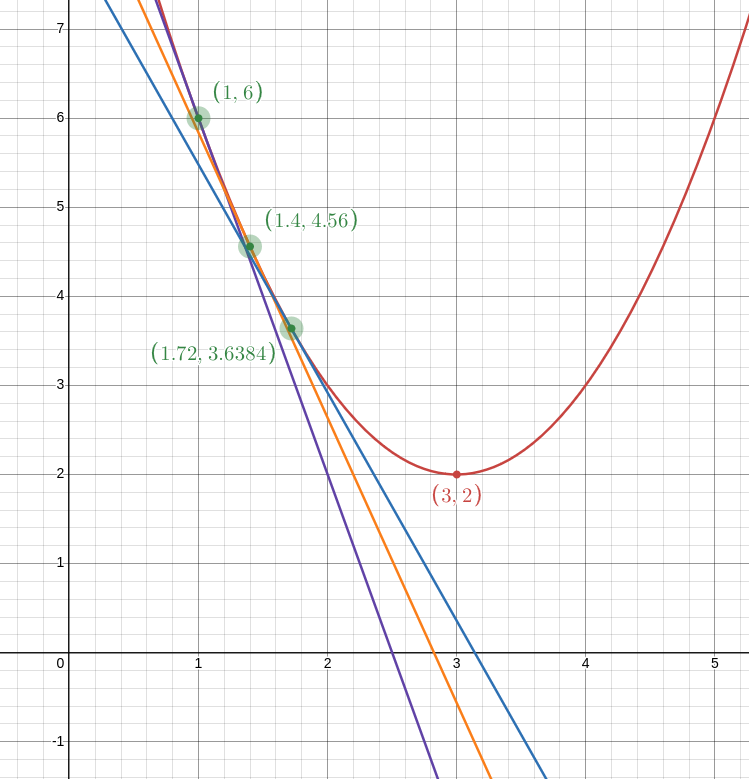
\includegraphics[width=0.5\textwidth]{gradient-descent-2d}
		\caption{Applying gradient descent to approximate the local minimum
		of $f(x) = 2 + (x - 3)^2$, starting at $x_0 = 1$.}
		\label{fig:gradient-descent-2d}
	\end{figure}
	The idea is that if we continue this way, we eventually arrive at $x_*$
	(assuming certain conditions on the function and the starting point).
	This is called \textbf{gradient descent}.
	\subsection*{Gradient Descent for Function of Multiple Variables}
	Let $f:\mathbb{R}^2\to\mathbb{R}$ be a scalar-valued function defined by
	\begin{align*}
		f(\bm{x}) = 2 + (x_1 - 3)^2 + (x_2 - 2)^4
	\end{align*}
	where $\bm{x} = \begin{bmatrix}
		x_1 & x_2
	\end{bmatrix}^\top$. We want to find the minimum at $\bm{x}_*=(3, 2)$. Analogous to
	the previous example, we compute the derivative, which in this case is
	the \textbf{gradient}:
	\begin{align*}
		\nabla f(\bm{x}) = \begin{bmatrix}
			\frac{\partial f}{\partial x_1}\\
			\frac{\partial f}{\partial x_2}
		\end{bmatrix}
		=
		\begin{bmatrix}
			2(x_1 - 3)\\
			4(x_2 - 2)^3
		\end{bmatrix}
	\end{align*}
	Let's use $\bm{x}_0 = \begin{bmatrix}
		1 & 1
	\end{bmatrix}^\top$
	as the starting point, and let $\eta = 0.1$. Then similar to before, we
	can approximate $\bm{x}_*$ by moving in the direction of $-\nabla f(\bm{x}_0)$.
	This works because the gradient of a scalar-valued function gives the direction
	of fastest rate of increase of a function. Thus, by moving in the direction
	of $-\nabla f(\bm{x}_0)$, we move in the direction of greatest decrease.
	We compute a first approximation to $\bm{x}_*$ as follows:
	\begin{align*}
		\bm{x}_1 &= \bm{x}_0 + (-\eta \cdot \nabla f(\bm{x}_0))
		= \begin{bmatrix}
			1\\
			1
		\end{bmatrix}
		- 0.1 \cdot \begin{bmatrix}
			-4\\
			-4
		\end{bmatrix}=
		\begin{bmatrix}
			1.4\\
			1.4
		\end{bmatrix}\\
		\vdots &= \vdots
	\end{align*}
	\section{Gradient Boosting}
	The \textbf{gradient boosting algorithm} is based on the idea of gradient descent.
	The reason it took so long to arrive at this algorithm is because it
	is more complicated. Instead of starting with a point, we start with
	a \textit{function}; each iteration we get not a new point but a new
	\textit{function}. We need two things to make this work:
	\begin{enumerate}[label=(\textbf{\arabic*})]
		\item A \textbf{loss function (error metric, objective function)}.
		We have seen many such functions throughout our study. Call this
		$L(\bm{y}, \hat{\bm{y}})$.
		\item Fit a model to the negative gradient of $L(\bm{y}, \hat{\bm{y}})$,
		that is to $-\nabla L(\bm{y}, \hat{\bm{y}})$,
		as the response.
	\end{enumerate}
	After many iterations, we see the loss decreases. Let's compare the
	notations for gradient boosting and gradient descent side-by-side:
	\begin{center}
		\begin{tabular}{|p{0.4\linewidth}|p{0.55\linewidth}|}
			\hline
			\textbf{Gradient Descent} & \textbf{Gradient Boosting}\\
			\hline
			Begin at $x_0$. &
			Begin at $G_0 := g_0$, the default (i.e., a the null model).\\
			\hline
			Direction to move: $-f'(x_0)$. &
			Move in the direction that improves loss. That is,
			run the algorithm on data $X$, but fit on loss of $\bm{y}$:
			\begin{align*}
				\mathcal{A}(\langle X, -\nabla L(\bm{y}, \hat{\bm{y}}_0) \rangle, \mathcal{H})
			\end{align*}\\
			\hline
			Move by amount $-\eta f'(x_0)$. &
			Move by amount
			\begin{align*}
				g_1 := \eta \mathcal{A}(\langle X, -\nabla L(\bm{y}, \hat{\bm{y}}_0)\rangle, \mathcal{H})
			\end{align*}\\
			\hline
			Compute a better approximation
			\begin{align*}
				x_1 := x_0 - \eta f'(x_0)
			\end{align*} &
			Compute a better approximation
			\begin{align*}
				G_1 := g_0 + g_1
			\end{align*}\\
			\hline
			Compute a second approximation
			\begin{align*}
				x_2 := x_1 - \eta f'(x_1)
			\end{align*} &
			Compute a second approximation
			\begin{align*}
				G_2 := \underbrace{g_0 + g_1}_{G_1} + \eta
				\mathcal{A}(\langle X, -\nabla L(\bm{y}, \hat{\bm{y}}_1)\rangle, \mathcal{H})
			\end{align*}\\
			\hline
			Compute $m$th approximation
			\begin{align*}
				x_m := x_{m-1} - \eta f'(x_{m-1})
			\end{align*} &
			Compute $m$th approximation
			\begin{align*}
				G_m := \underbrace{g_0 + g_1 + \cdots + g_{m-1}}_{G_{m-1}} + \eta
				\mathcal{A}(\langle X, -\nabla L(\bm{y}, \hat{\bm{y}}_{m-1})\rangle, \mathcal{H})
			\end{align*}\\
			\hline
		\end{tabular}
	\end{center}
	After $M$ steps, we set $g_{\text{boost}} = G_M$. The algorithm is the
	\textit{weak learner} that we talked about. Each term of $G_M$ gets better
	each time. In order to employ this algorithm, we need to know the loss function
	that we are trying to fit.
	\subsection*{Numeric Response Space, $\mathcal{Y} = \mathbb{R}$}
	Suppose we are predicting in a context where the response space is
	$\mathcal{Y} = \mathbb{R}$. For the loss function, we can use
	\begin{align*}
		L(\bm{y}, \hat{\bm{y}}) = SSE := \sum_{i=1}^{n}(y_i - \hat{y}_i)^2
	\end{align*}
	We compute the gradient by treating $L$ as a function of $\hat{\bm{y}}$
	(the output of the unknown prediction function), and we negate it:
	\begin{align*}
		-\nabla L(\bm{y}, \hat{\bm{y}})
		&=
		-\begin{bmatrix}
			\frac{\partial L}{\partial \hat{y}_1}\\
			\vdots\\
			\frac{\partial L}{\partial \hat{y}_n}
		\end{bmatrix}
		=-\begin{bmatrix}
			-(y_1 - \hat{y}_1)\\
			\vdots\\
			-(y_n - \hat{y}_n)
		\end{bmatrix}
		=2(\bm{y}-\hat{\bm{y}})
		=2\bm{e}
	\end{align*}
	where $\bm{e}$ is the residual vector. Thus, the algorithm begins by computing
	\begin{align*}
		g_1 := \eta \cdot \mathcal{A}(\langle X, 2\bm{e}\rangle, \mathcal{H})
	\end{align*}
	\subsection*{Probability Estimation, $\mathcal{Y} = \{0, 1\}$}
	Suppose we are predicting in a context where the response is space
	is $\mathcal{Y} = \{0, 1\}$, and we intend to use probability estimation.
	Our modeling target is $P(Y = 1 \mid \bm{x})$. Assume we use the logistic
	link function, which is
	\begin{align*}
		\phi(u) = \frac{e^u}{1 + e^u}
	\end{align*}
	We arrived at the following quantity for the probability of the data set
	$\mathbb{D}$ that we wished to maximize:
	\begin{align*}
		P(\bm{y}, \hat{\bm{p}}) = \prod_{i=1}^{n}\hat{p}_i^{y_i}(1-\hat{p}_i)^{1-y_i}
	\end{align*}
	where we have
	\begin{align*}
		\hat{p}_i = \phi(\hat{y}_i) = \frac{e^{\hat{y}_i}}{1 + e^{\hat{y}_i}}
		\iff
		\hat{y}_i = \ln  \left(\frac{\hat{p}_i}{1 - \hat{p}_i}\right)
	\end{align*}
	It turns out that it is easier to work with log-odds, so we will
	manipulate the equation for $P(\bm{y}, \hat{\bm{p}})$ to express
	it as a function of $\bm{y}$ and $\hat{\bm{y}}$:
	\begin{align*}
		P(\bm{y}, \hat{\bm{p}})
		&= \prod_{i=1}^{n}\hat{p}_i^{y_i}(1-\hat{p}_i)^{1-y_i}\\
		&= \prod_{i=1}^{n}
		\left(\frac{e^{\hat{y}_i}}{1 + e^{\hat{y}_i}}\right)^{y_i}\cdot
		\left(\frac{1}{1 + e^{\hat{y}_i}}\right)^{1 - y_i}
		\tag{Substitute expression for $\hat{p}_i$}\\
		&= \prod_{i=1}^{n} \frac{e^{y_i \hat{y}_i}}{1 + e^{\hat{y}_i}}\\
		&=P(\bm{y}, \hat{\bm{y}})
	\end{align*}
	Now recall that since the logistic link function is monotonically increasing,
	maximizing probability is equivalent to maximizing log-probability.
	We define the loss function $L(\bm{y}, \hat{\bm{y}})$ as
	\begin{align*}
		L(\bm{y}, \hat{\bm{y}})
		&=\ln(P(\bm{y}, \hat{\bm{y}}))\\
		&=\ln \left(\prod_{i=1}^{n} \frac{e^{y_i \hat{y}_i}}{1 + e^{\hat{y}_i}}\right)\\
		&=\sum_{i=1}^{n}\ln\left(\frac{e^{y_i \hat{y}_i}}{1 + e^{\hat{y}_i}}\right)
		\tag{Product property of logarithms}\\
		&=\sum_{i=1}^{n}(y_i\hat{y}_i - \ln(1 + e^{\hat{y}_i}))
		\tag{Quotient property of logarithms}
	\end{align*}
	Then we compute the negative gradient as before:
	\begin{align*}
		-\nabla L(\bm{y}, \hat{\bm{y}})
		= -\begin{bmatrix}
			\frac{\partial L}{\partial \hat{y}_1}\\
			\vdots\\
			\frac{\partial L}{\partial \hat{y}_n}
		\end{bmatrix}
		= -\begin{bmatrix}
			y_1 - \frac{e^{\hat{y}_1}}{1 + e^{\hat{y}_1}}\\
			\vdots\\
			y_n - \frac{e^{\hat{y}_n}}{1 + e^{\hat{y}_n}}
		\end{bmatrix}
		=\bm{y} - \hat{\bm{p}}
		=\bm{e}
	\end{align*}
	\section{Types of Machine Learning}
	Machine learning can be applied in a variety of ways. The following
	is a non-exhaustive survey of them.
	\subsection*{Machine Teaching}
	Begin with $\mathbb{D}$, and compute $g$. Then, inspect $\bm{e}$ 
	to see which $e_i$'s are large. Assume you can generate
	$\langle \bm{x}_*, y_*\rangle$, where $\bm{x}_* \approx \bm{x}_i$,
	and then retrain. The idea is to target specific places where residuals
	are poor.
	\subsection*{Supervised Learning}
	Use $\mathbb{D} = \langle X, \bm{y}\rangle$ to create $g$ for prediction.
	This was our focus this semester.
	\subsection*{Unsupervised Learning}
	Use $\mathbb{D} = X$ to \textit{understand} the covariate space. That is,
	we are not trying to \textit{predict}; we are trying to \textit{understand}.
	There are some variations on this idea:
	\begin{itemize}
		\item \textbf{Clustering}: Cluster units into groups $G_1,G_2,\ldots,G_K$,
		such that $G_1,\ldots,G_K$ form a partition of $X$
		(i.e., $\cup_{i=1}^{K}G_i = X$ and $G_i\cap G_j =\varnothing$ for $i\neq j$).
		\item \textbf{Anomaly detection}: Is a given $\bm{x}_*$ ``strange",
		considering the historical data $X$?
		\item \textbf{Dimension reduction}: Can you explain or approximate with
		much less than $p$ measurements? The main methods in this category are
		\textbf{principal component analysis (PCA)} and \textbf{factor analysis}.
	\end{itemize}
\end{document}